\jxhj{%教学后记
	}
\skrq{%授课日期
	}
\ktmq{%课题名称
	学习新内容 }
\jxmb{%教学目标,每行前面要加 \item
	\item 巩固上期的基本指令;

	\item 总结上期的编程思路;

	\item 总结机床的操作技巧;

	\item 了解本期的学习内容及学生情况;}
\jxzd{%教学重点,每行前面要加 \item
	\item 巩固上期的基本指令;

	\item 总结上期的编程思路;}
\jxnd{%教学难点,每行前面要加 \item
	\item 总结上期的编程思路;}
\jjff{%教学方法
	通过讲述、举例、演示法来说明;}

\makeshouye %制作教案首页

%%%%教学内容
\subsection{组织教学}
\begin{enumerate}[\hspace{2em}1、]
	\item 集中学生注意力;
	\item 清查学生人数;
	\item 维持课堂纪律;
\end{enumerate}
\subsection{复习导入及主要内容}
\begin{enumerate}[\hspace{2em}1、]
	\item 上学期末考试讲评;

	\item 了解学生情况;
\end{enumerate}
\subsection{教学内容及过程}
\subsubsection{本期教学安排} \marginpar{说明介绍}
\paragraph{理论教学计划:}
\begin{itemize}
	\item 复习上期内容

	\item 两面加工实例

	\item 变量与基本运算

	\item 椭圆加工if  goto

	\item 循环及其指令 if goto while

	\item 循环应用

	\item Siemens参数编程概述

	\item Siemens应用

	\item 镜象指令的使用

	\item 薄壁及配合件加工工艺

	\item 双曲线、抛物线加工

	\item 孔系加工(循环嵌套)

	\item 圆孔的宏程序

	\item 方槽椭圆槽的宏程序
	\item 斜面与圆柱面的宏程序

	\item 球面的宏程序(凸/凹)

	\item 椭球面的宏程序

	\item 任意轮廓倒圆角(系统变量)

	\item 任意轮廓倒圆角(G10)

	\item Siemens上倒角与倒圆

	\item 宏程序调用基本知识

	\item 宏程序调用的应用

	\item 多轴加工概述

	\item 四轴加工:圆柱凸轮的加工

	\item 五轴加工简介

	\item 综合练习(一)

	\item 综合练习(二)

	\item 综合练习(三)

	\item 综合练习(四)

\end{itemize}

\subparagraph{实习教学计划}
\begin{itemize}
	\item 两面加工类零件加工

	\item 薄壁配合件加工

	\item 宏程序加工

	\item 综合加工(钢材)
\end{itemize}

\subsubsection{手工编程复习} \marginpar{互动提问}
如下面的思维导图 \ref{手工编程思维导图}
\begin{figure}	
	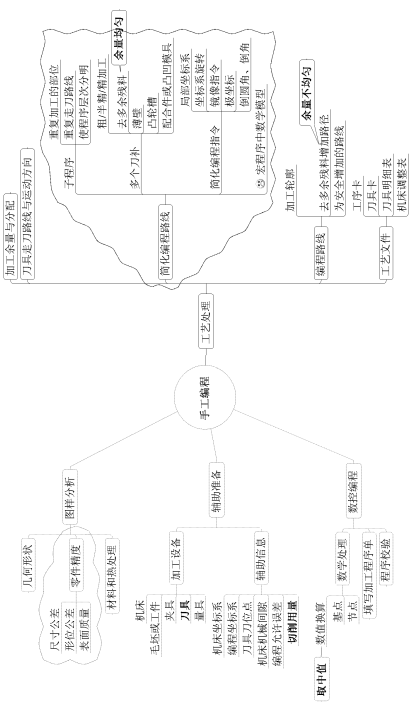
\includegraphics{images/图片1} 
	\caption{手工编程思维导图}\label{手工编程思维导图}
\end{figure}

\subsubsection{数控机床的操作}
如下面的思维导图 \ref{数控机床的操作思维导}
\begin{figure}	
	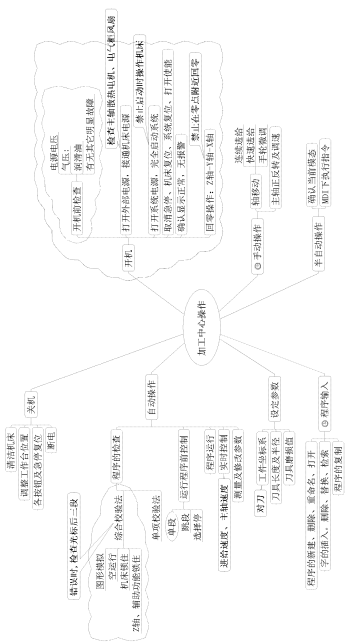
\includegraphics{images/图片2} 
	\caption{数控机床的操作思维导图} \label{数控机床的操作思维导}
\end{figure}

\subsubsection{数控机床指令}
\paragraph{G指令}\begin{itemize}
	\item G0 G1 G2 G3

	\item G17 G18 G19

	\item G9 G61 G62 G63 G64

	\item G4 

	\item G20 G21

	\item G40 G41 G42 

	\item G43 G44 G49

	\item G90 G91

	\item G98 G99

	\item G81 G82 G83 G84 G85 G86 G87 G88 G89 G80 G73 G74 G76

\end{itemize}

\paragraph{M指令}

\begin{itemize}
	\item M0 M1 M2 M30

	\item M3 M4 M5 M19

	\item M6 M7 M8 M9

	\item M98 M99

\end{itemize}

\paragraph{其它指令}
\subsubsection{常见加工结构}
\begin{itemize}
	\item 平面

	\item 外轮廓

	\item (岛屿)

	\item 孔
	\item 凸轮槽

	\item 复杂零件

	\item 配合零件

	\item CAD/CAM

	\item 宏程序

	\item 其它
\end{itemize}
\subsubsection{上学期期末试卷分析}
\subsection{课堂小结}
主要复习了数控方面的基本知识。
\vfill
\subsection{布置作业}
\begin{enumerate}[1、]
	\item 自选一零件图, 写出其工艺与程序.

	\item 写出如图所示零件的程序及与工艺.
\end{enumerate}